\documentclass[14pt]{extbook}
\usepackage{multicol, enumerate, enumitem, hyperref, color, soul, setspace, parskip, fancyhdr} %General Packages
\usepackage{amssymb, amsthm, amsmath, bbm, latexsym, units, mathtools} %Math Packages
\everymath{\displaystyle} %All math in Display Style
% Packages with additional options
\usepackage[headsep=0.5cm,headheight=12pt, left=1 in,right= 1 in,top= 1 in,bottom= 1 in]{geometry}
\usepackage[usenames,dvipsnames]{xcolor}
\usepackage{dashrule}  % Package to use the command below to create lines between items
\newcommand{\litem}[1]{\item#1\hspace*{-1cm}\rule{\textwidth}{0.4pt}}
\pagestyle{fancy}
\lhead{Progress Quiz 5}
\chead{}
\rhead{Version A}
\lfoot{9912-2038}
\cfoot{}
\rfoot{Spring 2021}
\begin{document}

\begin{enumerate}
\litem{
What is the domain of the function below?\[ f(x) = \sqrt[8]{-5 x - 9} \]\begin{enumerate}[label=\Alph*.]
\item \( (-\infty, a], \text{where } a \in [-1.6, 1] \)
\item \( (-\infty, \infty) \)
\item \( [a, \infty), \text{where } a \in [-1.4, 2.2] \)
\item \( (-\infty, a], \text{ where } a \in [-3.5, -1.6] \)
\item \( [a, \infty), \text{where } a \in [-2.4, -1] \)

\end{enumerate} }
\litem{
Choose the graph of the equation below.\[ f(x) = - \sqrt[3]{x + 8} - 4 \]\begin{enumerate}[label=\Alph*.]
\begin{multicols}{2}\item 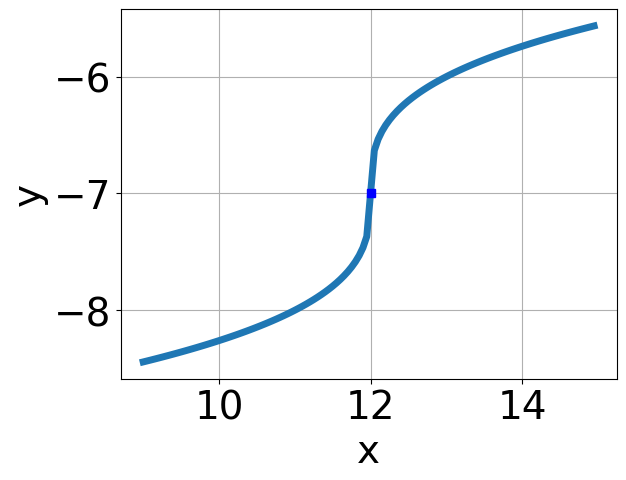
\includegraphics[width = 0.3\textwidth]{../Figures/radicalEquationToGraphAA.png}\item 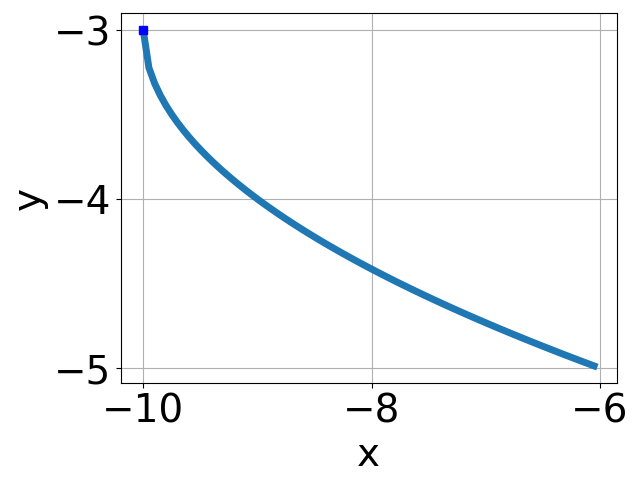
\includegraphics[width = 0.3\textwidth]{../Figures/radicalEquationToGraphBA.png}\item 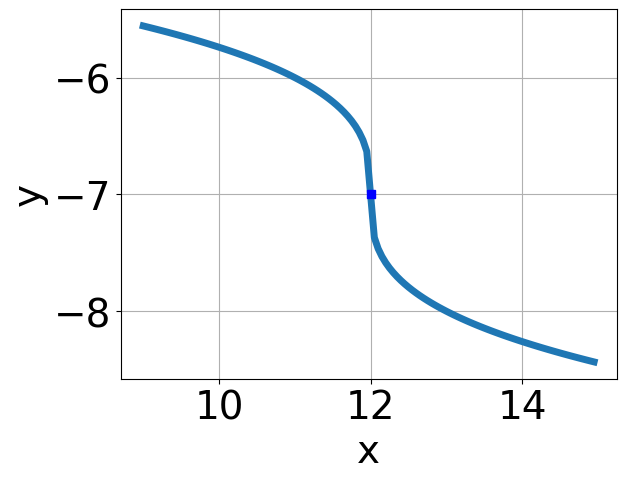
\includegraphics[width = 0.3\textwidth]{../Figures/radicalEquationToGraphCA.png}\item 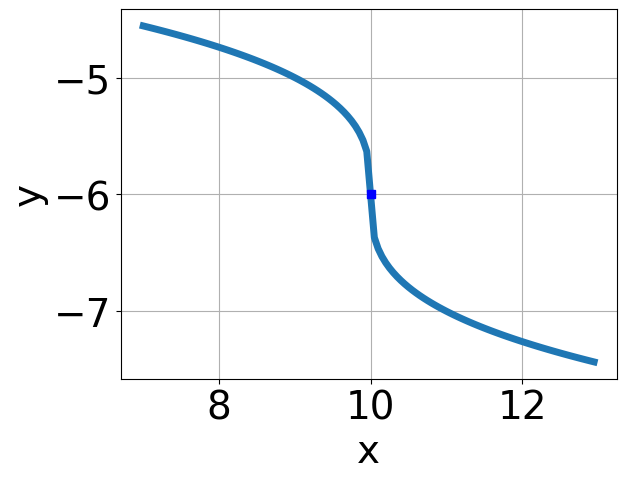
\includegraphics[width = 0.3\textwidth]{../Figures/radicalEquationToGraphDA.png}\end{multicols}\item None of the above.
\end{enumerate} }
\litem{
Solve the radical equation below. Then, choose the interval(s) that the solution(s) belongs to.\[ \sqrt{8 x + 4} - \sqrt{-9 x + 2} = 0 \]\begin{enumerate}[label=\Alph*.]
\item \( x \in [-0.32,0.05] \)
\item \( x_1 \in [-0.71, -0.48] \text{ and } x_2 \in [-0.62,0.07] \)
\item \( x \in [-0.38,-0.24] \)
\item \( \text{All solutions lead to invalid or complex values in the equation.} \)
\item \( x_1 \in [-0.71, -0.48] \text{ and } x_2 \in [0.13,0.86] \)

\end{enumerate} }
\litem{
Solve the radical equation below. Then, choose the interval(s) that the solution(s) belongs to.\[ \sqrt{-24 x^2 - 32} - \sqrt{76 x} = 0 \]\begin{enumerate}[label=\Alph*.]
\item \( x \in [-2.9,-1.5] \)
\item \( x \in [-2.4,2.6] \)
\item \( \text{All solutions lead to invalid or complex values in the equation.} \)
\item \( x_1 \in [2.3, 2.9] \text{ and } x_2 \in [-0.48,0.97] \)
\item \( x_1 \in [-2.9, -1.5] \text{ and } x_2 \in [-1.23,0.15] \)

\end{enumerate} }
\litem{
Solve the radical equation below. Then, choose the interval(s) that the solution(s) belongs to.\[ \sqrt{-2 x - 6} - \sqrt{9 x - 9} = 0 \]\begin{enumerate}[label=\Alph*.]
\item \( x_1 \in [-3.27, -2.09] \text{ and } x_2 \in [0.56,1.22] \)
\item \( \text{All solutions lead to invalid or complex values in the equation.} \)
\item \( x \in [-0.58,0.96] \)
\item \( x_1 \in [-3.27, -2.09] \text{ and } x_2 \in [-0.41,0.75] \)
\item \( x \in [-2.25,-1.11] \)

\end{enumerate} }
\litem{
Choose the graph of the equation below.\[ f(x) = \sqrt[3]{x - 14} + 5 \]\begin{enumerate}[label=\Alph*.]
\begin{multicols}{2}\item 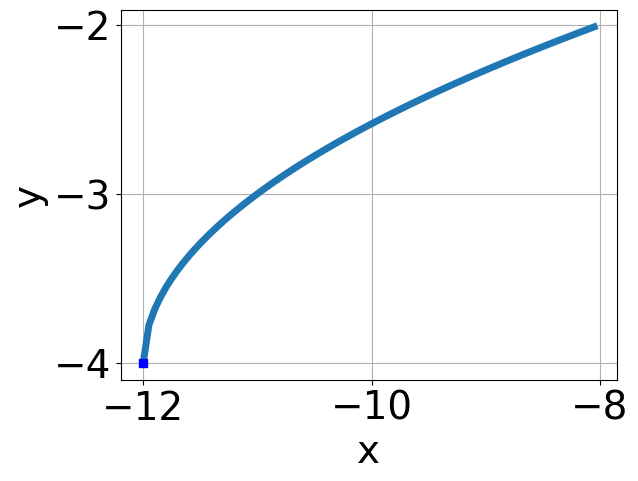
\includegraphics[width = 0.3\textwidth]{../Figures/radicalEquationToGraphCopyAA.png}\item 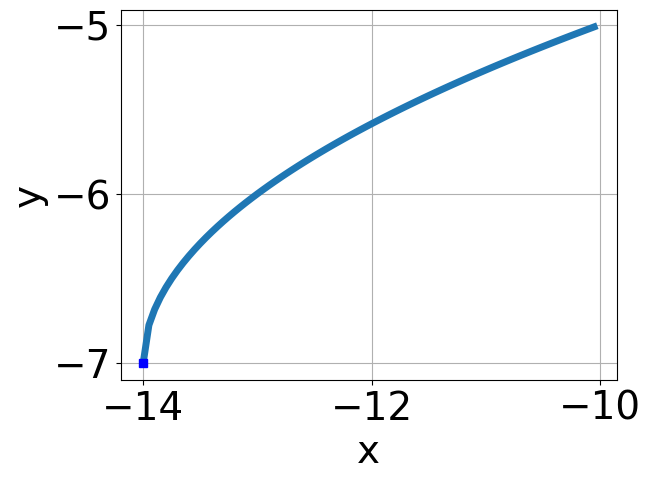
\includegraphics[width = 0.3\textwidth]{../Figures/radicalEquationToGraphCopyBA.png}\item 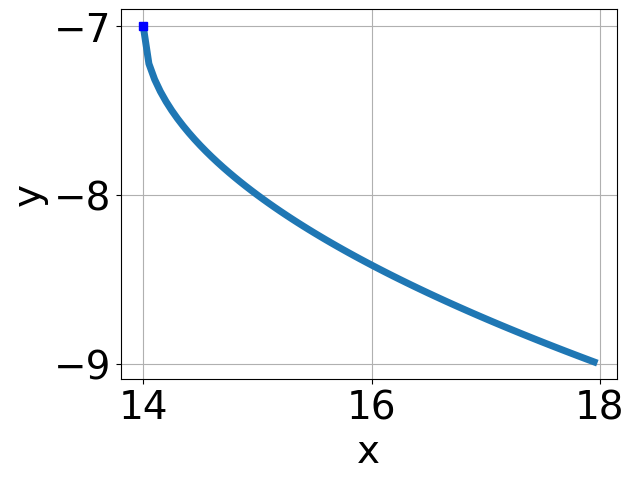
\includegraphics[width = 0.3\textwidth]{../Figures/radicalEquationToGraphCopyCA.png}\item 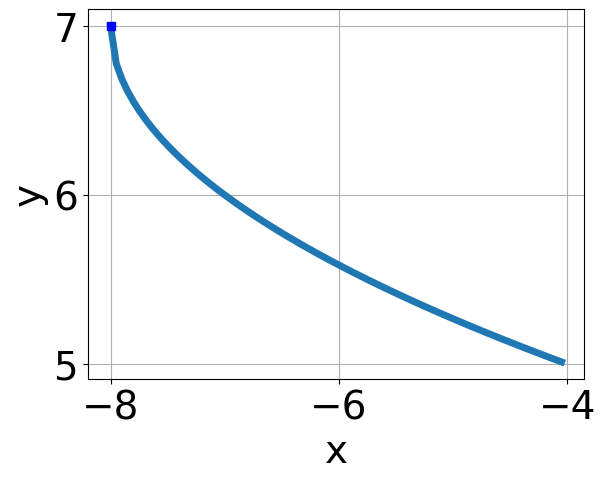
\includegraphics[width = 0.3\textwidth]{../Figures/radicalEquationToGraphCopyDA.png}\end{multicols}\item None of the above.
\end{enumerate} }
\litem{
Choose the equation of the function graphed below.
\begin{center}
    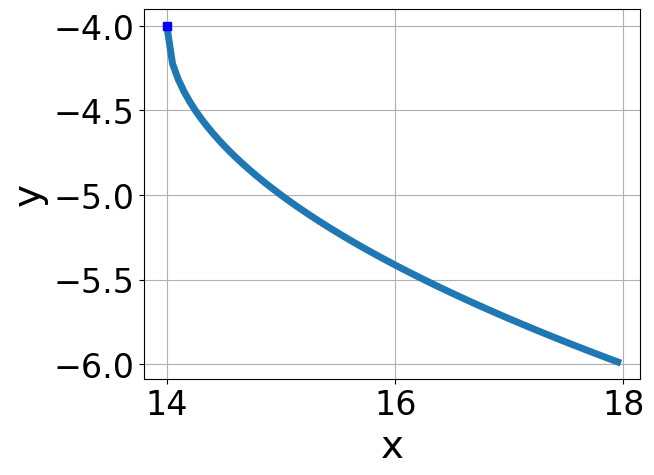
\includegraphics[width=0.5\textwidth]{../Figures/radicalGraphToEquationCopyA.png}
\end{center}
\begin{enumerate}[label=\Alph*.]
\item \( f(x) = - \sqrt[3]{x + 6} - 5 \)
\item \( f(x) = - \sqrt[3]{x - 6} - 5 \)
\item \( f(x) = \sqrt[3]{x + 6} - 5 \)
\item \( f(x) = \sqrt[3]{x - 6} - 5 \)
\item \( \text{None of the above} \)

\end{enumerate} }
\litem{
Solve the radical equation below. Then, choose the interval(s) that the solution(s) belongs to.\[ \sqrt{6 x^2 + 42} - \sqrt{33 x} = 0 \]\begin{enumerate}[label=\Alph*.]
\item \( x_1 \in [1.4, 3.1] \text{ and } x_2 \in [-0.5,6.5] \)
\item \( x \in [1.4,3.1] \)
\item \( x_1 \in [-4.9, -2.4] \text{ and } x_2 \in [-3,1] \)
\item \( \text{All solutions lead to invalid or complex values in the equation.} \)
\item \( x \in [2.3,4] \)

\end{enumerate} }
\litem{
What is the domain of the function below?\[ f(x) = \sqrt[8]{7 x - 9} \]\begin{enumerate}[label=\Alph*.]
\item \( [a, \infty), \text{ where } a \in [1.21, 1.95] \)
\item \( (-\infty, \infty) \)
\item \( [a, \infty), \text{where } a \in [0.76, 1.05] \)
\item \( (-\infty, a], \text{where } a \in [0.59, 1.23] \)
\item \( (-\infty, a], \text{where } a \in [0.99, 2.9] \)

\end{enumerate} }
\litem{
Choose the equation of the function graphed below.
\begin{center}
    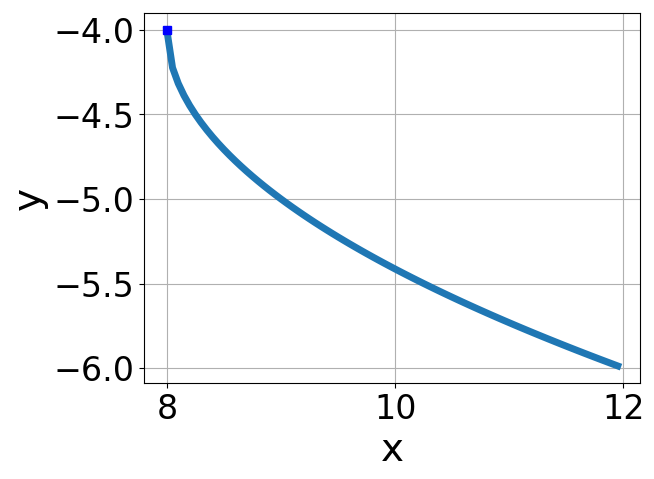
\includegraphics[width=0.5\textwidth]{../Figures/radicalGraphToEquationA.png}
\end{center}
\begin{enumerate}[label=\Alph*.]
\item \( f(x) = \sqrt{x - 10} - 7 \)
\item \( f(x) = \sqrt{x + 10} - 7 \)
\item \( f(x) = - \sqrt{x + 10} - 7 \)
\item \( f(x) = - \sqrt{x - 10} - 7 \)
\item \( \text{None of the above} \)

\end{enumerate} }
\end{enumerate}

\end{document}